\pagestyle{empty}
\section{Electromagnetismo}

\info{Contenido}{Electromagnetismo:imanes, campo eléctrico, electricidad, electrones y polaridad}

\subsection{Imanes}
\info{Imanes}{Son cuerpos que poseen la capacidad, propiedad de atraer al hierro.}

\begin{itemize}
    \item Imanes Naturales: Son minerales de hierro \emph{magenetita}, que se encuentran en la naturaleza.
    \item Imanes Artificiales: Son piezas de hierro que adquieren propiedades magnéticas.
    \item Imanes Temporales: Son todos los construidos por hierro dulce ( aleación de hierro-carbono con el 0,2\% de carbono, que pierden sus propiedades magnéticas si se va la causa imanadora.
    \item Imanes permanentes: Son todos los constituidos por acero ( aleación de hierro-carbono con el 0,2\% de carbono.
\end{itemize}

\subsection{Polos y líneas neutras de un imán}

Los imanes poseen la propiedad de atraer al hierro de forma intensa en sus polos. Se denomina polo norte $N$ aquel que si el imán puede moverse hacia el norte geográfico. No es posible aislar el polo único, cada imán tiene su polo norte $N$ y sur $S$, además posee la zona denominada línea neutra que es el centro del imán, en este centro los efectos magnéticos son nulos.

\subsection{Acción mutua entre imanes}

Los imanes del mismo polo se repelen y de distintos se atraen.

\subsection{Campo magnético}

Es la región del espacio donde se hacen sensibles las fuerzas o acciones magnéticas.

\subsection{Líneas de fuerza}

EL campo magnético se representa por líneas cerradas, llamadas líneas de fuerza a las que se le dá un sentido. En el imán las líneas de fuerza salen por el polo norte y entran al por el sur.

Las secciones magnéticas son más intensas donde la línea de fuerzas están más juntas.


\begin{center}
    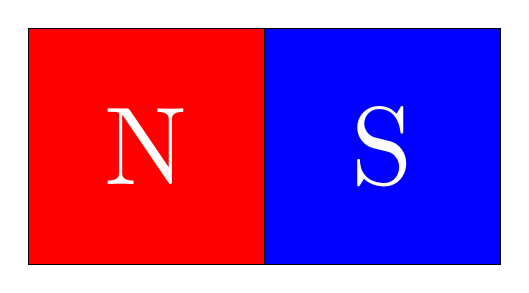
\begin{tikzpicture}
    \path [fill=red] (0,0)--(3,0)--(3,3)--(0,3)--(0,0);
    \path [fill=blue] (3,0)--(3,3)--(6,3)--(6,0)--(3,0);
    
    \draw (0,0) rectangle (6,3);
    \draw (3,0)--(3,3);
    \draw [color=white](1.5,1.5) node[scale=4]{N};
    \draw [color=white](4.5,1.5) node[scale=4]{S};
    
    \end{tikzpicture}
\end{center}

\subsection{Campo magnético creado por una corriente eléctrica rectilínea}

La corriente eléctrica al circular por un conductor rectilíneo alrededor de un campo magnético con las líneas de fuerza son circunferencias concéntricas, en cada plano perpendicular al conductor, y sus sentidos es el que corresponde al giro de un sacacorchos que avanza al sentido de la corriente.

\subsection{Campo magnético de una espira.}

Si se dobla un conductor recto por donde circula la corriente formando un trazo a espira, el campo magnético aumenta porque las líneas de fuerza se concentran en el centro de la espira. El campo magnético en el interior de la espira es perpendicular al plano de la misma y su sentido viene dado por el avance del sacacorchos que gira en el sentido de la corriente.

\subsection{Campo magnético de una bobina}

Para reforzar el campo magnético de una espira se dobla el conductor formando varias espiras sucesivas, lo que constituye una bobina. El campo magnético en el interior de la bobina es perpendicular al plano de las espiras y viene dado por el sentido del avance de un sacacorchos que gira en el sentido de la corriente.

\subsection{Inducción magnética}

Es el número de líneas de fuerzas del campo magnético por unidad de superficie perpendicular a dichas líneas.  En el sistema C.G.S. cada línea representa una unidad de inducción.
La inducción magnética es representada con la letra $B$.

\subsection{Unidades de inducción magnética.}

En el sistema internacional de unidades, la unidad de inducción es el Tesla $[T]$.

En el sistema C.G.S. la unidad es el Gauss [Gs] 

\begin{equation*}
    1T=10^4Gs
\end{equation*}

\subsection{Inducción magnética en el interior de un solenoide.}

Una bobina cuya longitud es mayor que su radio se llama solenoide. la inducción magnética en el interior de un solenoide es:

\info{Inducción en un solenoide}{
\begin{equation*}
 B=\frac{\mu \times N \times I}{l}   
\end{equation*}
siendo:

$B$: inducción magnética en teslas $[T]$.

$N$: Número de espiras.

$I$: Intensidad de la corriente en amperes $[A]$.

$l$: Longitud del solenoide en metros $[m]$

$\mu$ permeabilidad magnética del material del interior del solenoide. $[\frac{Tm}{A}]$.

En el sistema internacional de unidades y en el vacío o aire.

\begin{equation*}
    \mu = 4 \times \pi \times 10^{-7}= \frac{12,56 T \cdot m}{10^7 A} 
\end{equation*}

}

\subsection{Flujo Magnético $\Phi$}

El flujo magnético a través de una superficie es el número total de líneas de fuerza que atraviesan dicha superficie.
El flujo magnético se representa con la letra griega $\Phi$.
En un campo magnético uniforme el flujo a través de una superficie perpendicular a las líneas de fuerzas es el producto de la inducción por la superficie.

\subsection {Unidades de flujo magnético}

En el $SI$ sistema internacional, la unidad de flujo es el $Weber$ $[Wb]$.

En el sistema $C.G.S.$ es el $Maxell$ $[MX]$

La relación entre estas unidades es la siguiente $1WB = 10^8Mx$.

\subsection{Intensidad de campo magnético $B$}

La intensidad de campo magnético $H$ es la relación entre la inducción magnética $B$ y la permeabilidad $\mu$, del medio material en que el se ha establecido.

La intensidad de campo magnético se representa $H= \frac{B}{\mu}$.

\subsubsection{Intensidad de campo magnético en el interior de un solenoide}

La intensidad del campo magnético dentro de un solenoide por el que circula una corriente son los amperios-vuelta por unidad de longitud.
\begin{equation*}
    H=\frac{N \times I}{l}
\end{equation*}

Siendo:

$H$: Intensidad de campo magnético$ [frac{Av}{m}]$.

$N$: Número de espiras o vueltas.

$I$: Intensidad de corriente $[A]$.

$l$: Longitud del solenoide $[H]$.

\subsection{Sustancias ferromagnéticas}

Son sustancias con permeabilidad $\mu$ mucho mayor al vacío y dependiente de la inducción magnética $B$ ( Hierro, cobalto, niquel, sus aleaciones con carbono y otro metales). Estas sustancias son fuertemente atraídas por un iman.

La permeabilidad de estas sustancias se calcula multiplicando la permeabilidad del aire por un coeficiente llamado permeabilidad relativa.
\begin{equation}
    \mu=\mu_r \times \mu_0
\end{equation}

Siendo:

$\mu$: Permeabilidad absoluta.

$\mu_0$: Permeabilidad del vacío o del aire $\mu_0 = 4 \pi \times 10^{-7} \frac{Tm}{A}$

$\mu$: Permeabilidad relativa [adimensional].

\subsection{Teoría molecular de los imanes}

Se admite que las sustancias ferromagnéticas están constituídas por moléculas magnéticas o imanes elementales llamados \emph{dominios magnéticos}.

Antes de haber sometido la sustancia a la acción de un campo magnética, exterior, los imanes moleculares están perfectamente desorientados y mediante un campo magnético exterior se orientan, cuando más intensa sea la intensidad del campo magnetizante, hasta que todos los imanes elementales estén orientados que es el estado de saturación magnética.
Al cesar la acción magnetizante exterior los imanes moleculares pueden desorientarse como por ejemplo el caso de hierro dulce, perdiendo el material sus propiedades magnéticas o quedando orientados como en el caso del acero y conservando sus propiedades magnéticas.

%\subsection{Histéresis magnética}
